\documentclass[aspectratio=169,xcolor=dvipsnames]{beamer}
\usepackage{booktabs}
\usepackage{array}
\usepackage{multirow}
\usepackage{graphicx}
\usepackage{tikz}
\usetikzlibrary{shapes.geometric}
\usepackage{amsmath}
\usepackage{xcolor}
\usepackage{adjustbox}
\usepackage{tabularx}

% Simple academic theme
\usetheme{default}
\usecolortheme{default}

% Conservative academic color scheme
\definecolor{darkblue}{RGB}{25,25,112}
\definecolor{darkgray}{RGB}{64,64,64}
\definecolor{mediumgray}{RGB}{128,128,128}

% Set simple beamer colors
\setbeamercolor{titlelike}{fg=darkblue}
\setbeamercolor{structure}{fg=darkblue}
\setbeamercolor{normal text}{fg=black}
\setbeamercolor{alerted text}{fg=darkgray}
\setbeamercolor{example text}{fg=darkgray}

% Font configurations
\setbeamerfont{title}{size=\Large,series=\bfseries}
\setbeamerfont{subtitle}{size=\large}
\setbeamerfont{author}{size=\normalsize}
\setbeamerfont{frametitle}{size=\Large,series=\bfseries}

% Simple custom commands
\newcommand{\highlight}[1]{\textbf{#1}}
\newcommand{\success}[1]{\textcolor{darkgray}{\textbf{#1}}}
\newcommand{\emphasis}[1]{\textcolor{darkblue}{\textbf{#1}}}

% Title information
\title{Towards Energy-Aware AI Deployment}
\subtitle{Investigating the Interplay of Model Quantization and Hardware Platforms}
\author{Haoji Bian \and Zinan Wang \and Renyuan Lu}
\institute{Northwestern University}
\date{\today}

% Remove navigation symbols
\setbeamertemplate{navigation symbols}{}

% Add page numbers
\setbeamertemplate{footline}[frame number]

\begin{document}

%% Slide 1: Title Page (10 seconds)
\begin{frame}
\titlepage
\end{frame}

%% Slide 2: Research Motivation (25 seconds)
\begin{frame}
\frametitle{Research Motivation}

\begin{columns}[c]
\column{0.5\textwidth}
\begin{block}{Energy Challenge in LLMs}
\begin{itemize}
\item Training a large Transformer: \highlight{1,287,000 kWh}
\item Equivalent to lifetime emissions of multiple vehicles
\item Growing inference demands in production systems
\end{itemize}
\end{block}

\vspace{0.5cm}
\begin{alertblock}{Research Gap}
Inference-stage energy optimization receives insufficient attention despite its critical importance in deployment scenarios.
\end{alertblock}

\column{0.5\textwidth}
\begin{figure}
\centering
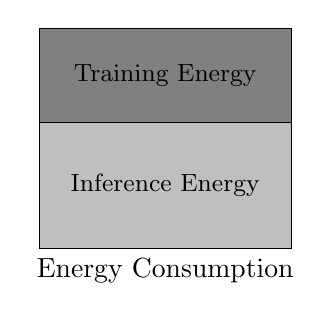
\begin{tikzpicture}[scale=0.8]
\draw[fill=lightgray] (0,0) rectangle (4,2);
\draw[fill=gray] (0,2) rectangle (4,3.5);
\node at (2,1) {\small Inference Energy};
\node at (2,2.75) {\small Training Energy};
\node[below] at (2,0) {Energy Consumption};
\end{tikzpicture}
\caption{LLM Energy Distribution}
\end{figure}

\end{columns}
\end{frame}

%% Slide 3: Research Question (25 seconds)
\begin{frame}
\frametitle{Core Research Question}

\begin{center}
\begin{beamercolorbox}[wd=0.9\textwidth,center]{structure}
\Large\textbf{How can we achieve energy-efficient LLM deployment through systematic optimization of \highlight{quantization techniques} and \highlight{hardware platforms}?}
\end{beamercolorbox}
\end{center}

\vspace{1cm}

\begin{columns}[c]
\column{0.48\textwidth}
\begin{block}{Existing Limitations}
\begin{itemize}
\item Focus on isolated optimization factors
\item Lack of systematic evaluation frameworks
\item Limited deployment guidance
\end{itemize}
\end{block}

\column{0.48\textwidth}
\begin{exampleblock}{Our Contribution}
\begin{itemize}
\item Systematic co-optimization approach
\item Comprehensive evaluation framework
\item Practical deployment guidelines
\end{itemize}
\end{exampleblock}

\end{columns}
\end{frame}

%% Slide 4: Methodology Overview (30 seconds)
\begin{frame}
\frametitle{Methodology: Three-Pillar Approach}

\begin{columns}[c]
\column{0.32\textwidth}
\begin{block}{Pillar 1: Quantization Analysis}
\begin{center}
\begin{itemize}
\item INT8, FP16, Dynamic quantization
\item Performance-energy trade-offs
\item Memory optimization
\end{itemize}
\end{center}
\end{block}

\column{0.32\textwidth}
\begin{block}{Pillar 2: Hardware Evaluation}
\begin{center}
\begin{itemize}
\item 6 GPU platforms
\item 3 hardware generations
\item Comprehensive energy profiling
\end{itemize}
\end{center}
\end{block}

\column{0.32\textwidth}
\begin{block}{Pillar 3: Energy Metrics}
\begin{center}
\begin{itemize}
\item Novel EOR/TWEOR metrics
\item 1Hz precision monitoring
\item Deployment optimization
\end{itemize}
\end{center}
\end{block}

\end{columns}

\vspace{0.8cm}
\begin{center}
\begin{beamercolorbox}[wd=0.9\textwidth,center]{structure}
\textbf{Systematic Co-optimization Framework: 6 Platforms × 6 Models × 5 Tasks}
\end{beamercolorbox}
\end{center}
\end{frame}

%% Slide 5: Energy Efficiency Metrics (30 seconds)
\begin{frame}
\frametitle{Novel Energy Efficiency Metrics}

\begin{columns}[c]
\column{0.6\textwidth}

\begin{block}{Energy Output Ratio (EOR)}
$$EOR = \frac{\text{Performance Score}}{\text{Energy (Wh)}}$$
\end{block}

\vspace{0.5cm}

\begin{block}{Time-Weighted Energy Output Ratio (TWEOR)}
Incorporates both energy consumption and inference time for comprehensive efficiency evaluation
\end{block}

\column{0.4\textwidth}
\begin{exampleblock}{Metric Advantages}
\begin{itemize}
\item Captures complex trade-offs
\item Incorporates temporal efficiency
\item Enables deployment optimization
\end{itemize}
\end{exampleblock}

\vspace{0.5cm}
\begin{alertblock}{Data Collection}
NVIDIA SMI\\
1Hz sampling rate\\
Precise energy measurements
\end{alertblock}

\end{columns}
\end{frame}

%% Slide 6: Experimental Setup (30 seconds)
\begin{frame}
\frametitle{Experimental Configuration}

\begin{columns}[c]
\column{0.45\textwidth}
\begin{block}{Hardware \& Models}
\textbf{6 GPU Platforms:} A100, RTX 4090/3090Ti/4060Ti, V100, L40S\\
\textbf{6 Language Models:} Qwen2.5, DeepSeek-R1, Mistral, Neural-Chat, Bloomz, Yi\\
\textbf{3 Quantization:} INT8, FP16, Dynamic
\end{block}

\column{0.55\textwidth}
\begin{block}{Benchmark Tasks}
\begin{itemize}
\item \textbf{MMLU}: Multi-task language understanding
\item \textbf{HellaSwag}: Commonsense reasoning
\item \textbf{ARC}: Science question answering
\item \textbf{TruthfulQA}: Truthfulness evaluation
\item \textbf{GSM8K}: Mathematical reasoning
\end{itemize}
\end{block}

\begin{figure}
\centering
\includegraphics[width=\textwidth]{img/System_Memory_Usage.png}
\caption{System Resource Monitoring}
\end{figure}

\end{columns}

\vspace{0.3cm}
\begin{center}
\begin{beamercolorbox}[wd=\textwidth,center]{structure}
\textbf{Comprehensive Evaluation: 6 Platforms × 6 Models × 5 Benchmark Tasks}
\end{beamercolorbox}
\end{center}
\end{frame}

%% Slide 7: Finding 1 - Quantization Impact (60 seconds)
\begin{frame}
\frametitle{Finding 1: Quantization Techniques Effectiveness}

\begin{table}[h]
\centering
\begin{tabular}{@{}lcccc@{}}
\toprule
\textbf{Strategy} & \textbf{Energy Red.} & \textbf{Acc. Loss} & \textbf{EOR Imp.} & \textbf{Rating} \\
\midrule
INT8 Quantization & \textbf{25.0\%} & <1.0\% & \textbf{32.1\%} & Excellent \\
FP16 Mixed Precision & 16.3\% & 0.2\% & 19.4\% & Good \\
Dynamic Quantization & 10.5\% & 1.5\% & 11.7\% & Moderate \\
\bottomrule
\end{tabular}
\end{table}

\begin{columns}[c]
\column{0.6\textwidth}
\begin{exampleblock}{INT8 Quantization Results}
\begin{itemize}
\item DeepSeek-7B: \textbf{39.65Wh → 29.74Wh}
\item Accuracy degradation: 0.7-0.9 percentage points
\item Reduced memory bandwidth requirements
\item Optimized integer arithmetic on modern GPUs
\end{itemize}
\end{exampleblock}

\column{0.4\textwidth}
\begin{figure}
\centering
\includegraphics[width=\textwidth]{img/Result_Analysis_Algorithm.png}
\caption{Quantization Trade-offs}
\end{figure}

\end{columns}
\end{frame}

%% Slide 8: Finding 2a - A100 Leadership (30 seconds)
\begin{frame}
\frametitle{Finding 2a: A100 PCIE Leadership}

\begin{center}
\begin{beamercolorbox}[wd=0.8\textwidth,center]{structure}
\Large\textbf{A100 PCIE: Energy Efficiency Champion}
\end{beamercolorbox}
\end{center}

\vspace{0.5cm}

\begin{columns}[c]
\column{0.5\textwidth}
\begin{exampleblock}{Technical Specifications}
\begin{itemize}
\item \textbf{Memory Bandwidth}: 1,555 GB/s
\item \textbf{Tensor Cores}: 3rd generation
\item \textbf{Memory}: 40GB HBM2
\item \textbf{Architecture}: Ampere
\end{itemize}
\end{exampleblock}

\column{0.5\textwidth}
\begin{block}{Performance Leadership}
\begin{itemize}
\item \textbf{Highest energy efficiency} across all scenarios
\item Optimized for AI workloads
\item Superior memory bandwidth utilization
\item Enterprise-grade reliability
\end{itemize}
\end{block}

\end{columns}

\vspace{0.5cm}
\begin{center}
\begin{beamercolorbox}[wd=0.9\textwidth,center]{example text}
\textbf{Consistent leader in EOR and TWEOR metrics across all benchmark tasks}
\end{beamercolorbox}
\end{center}
\end{frame}

%% Slide 9: Finding 2b - Platform Analysis (30 seconds)
\begin{frame}
\frametitle{Finding 2b: Hardware Platform Analysis}

\begin{columns}[c]
\column{0.4\textwidth}
\begin{block}{Platform Categories}
\begin{itemize}
\item \textbf{High bandwidth}: A100, V100
\item \textbf{Power optimized}: RTX 4060Ti
\item \textbf{High-performance}: RTX 4090
\end{itemize}
\end{block}

\vspace{0.5cm}
\begin{exampleblock}{Ada Lovelace Architecture}
\textbf{20-30\%} energy efficiency improvement over previous generation
\end{exampleblock}

\column{0.6\textwidth}
\begin{figure}
\centering
\includegraphics[width=\textwidth]{img/overall_performance_heatmap.png}
\caption{Platform Performance Heatmap}
\end{figure}

\end{columns}
\end{frame}

%% Slide 10: Finding 3 - Synergistic Optimization (60 seconds)
\begin{frame}
\frametitle{Finding 3: Synergistic Optimization Effects}

\begin{center}
\begin{beamercolorbox}[wd=0.8\textwidth,center]{structure}
\Large\textbf{40\% Overall Energy Efficiency Improvement}\\
\normalsize A100 PCIE + INT8 Quantization
\end{beamercolorbox}
\end{center}

\vspace{0.5cm}

\begin{columns}[c]
\column{0.5\textwidth}
\begin{table}[h]
\centering
\footnotesize
\begin{tabular}{@{}lc@{}}
\toprule
\textbf{Optimization Strategy} & \textbf{Efficiency Gain} \\
\midrule
A100 + INT8 & \textbf{40.0\%} \\
RTX 4090 + FP16 & \textbf{35.2\%} \\
RTX 4060Ti + Dynamic & 25.1\% \\
\bottomrule
\end{tabular}
\end{table}

\column{0.5\textwidth}
\begin{exampleblock}{Additional Benefits}
\begin{itemize}
\item \textbf{Knowledge Distillation}: Additional \textbf{19.8\%} energy reduction
\item \textbf{Accuracy Preservation}: Maintains \textbf{98\%+} performance
\end{itemize}
\end{exampleblock}

\end{columns}

\vspace{0.3cm}
\begin{center}
\begin{beamercolorbox}[wd=\textwidth,center]{example text}
\Large\textbf{Hardware-software co-optimization enables multiplicative benefits}
\end{beamercolorbox}
\end{center}
\end{frame}

%% Slide 11: Deployment Guidelines (30 seconds)
\begin{frame}
\frametitle{Deployment Decision Flow}

\begin{center}
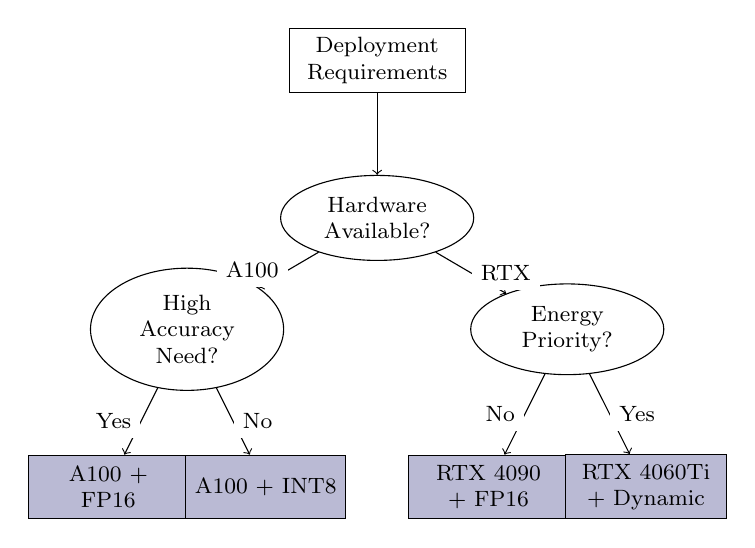
\begin{tikzpicture}[node distance=2cm, 
    every node/.style={fill=white, font=\footnotesize},
    decision/.style={ellipse, draw, text width=1.5cm, text centered, minimum height=1cm},
    process/.style={rectangle, draw, text width=2cm, text centered, minimum height=0.8cm},
    endpoint/.style={rectangle, draw, fill=darkblue!30, text width=1.8cm, text centered, minimum height=0.8cm}]

% Start
\node[process] (start) {Deployment Requirements};

% Decision 1
\node[decision, below of=start] (hardware) {Hardware Available?};

% Decision 2  
\node[decision, below left of=hardware, xshift=-1cm] (accuracy) {High Accuracy Need?};

% Decision 3
\node[decision, below right of=hardware, xshift=1cm] (energy) {Energy Priority?};

% Endpoints
\node[endpoint, below of=accuracy, xshift=-1cm] (fp16) {A100 + FP16};
\node[endpoint, below of=accuracy, xshift=1cm] (int8) {A100 + INT8};
\node[endpoint, below of=energy, xshift=-1cm] (rtx) {RTX 4090 + FP16};
\node[endpoint, below of=energy, xshift=1cm] (edge) {RTX 4060Ti + Dynamic};

% Arrows
\draw[->] (start) -- (hardware);
\draw[->] (hardware) -- node[left] {A100} (accuracy);
\draw[->] (hardware) -- node[right] {RTX} (energy);
\draw[->] (accuracy) -- node[left] {Yes} (fp16);
\draw[->] (accuracy) -- node[right] {No} (int8);
\draw[->] (energy) -- node[left] {No} (rtx);
\draw[->] (energy) -- node[right] {Yes} (edge);

\end{tikzpicture}
\end{center}

\vspace{0.5cm}
\begin{center}
\begin{beamercolorbox}[wd=0.9\textwidth,center]{structure}
\textbf{Systematic Decision Process: Assessment → Analysis → Consideration → Optimization}
\end{beamercolorbox}
\end{center}
\end{frame}

%% Slide 12: Deployment Decision Matrix (30 seconds)
\begin{frame}
\frametitle{Deployment Decision Matrix}

\begin{table}[h]
\centering
\scriptsize
\begin{tabular}{@{}lccccc@{}}
\toprule
\textbf{Use Case} & \textbf{Hardware} & \textbf{Quantization} & \textbf{Performance} & \textbf{Efficiency Gain} & \textbf{Cost} \\
\midrule
Data Center Production & A100 PCIE & INT8 & 98\% & \textbf{40\%} & High \\
Enterprise Applications & RTX 4090 & FP16 & 99\% & \textbf{35\%} & Medium-High \\
R\&D Testing & RTX 3090Ti & FP16 & 97\% & 30\% & Medium \\
Edge Computing & RTX 4060Ti & Dynamic & 95\% & 25\% & Low \\
Budget-Constrained & V100 & INT8 & 94\% & 28\% & Low \\
\bottomrule
\end{tabular}
\end{table}

\begin{columns}[c]
\column{0.4\textwidth}
\begin{exampleblock}{Selection Principles}
\begin{itemize}
\item \textbf{Accuracy Priority} → FP16 mixed precision
\item \textbf{Energy Priority} → INT8 quantization
\item \textbf{Flexibility Priority} → Dynamic quantization
\end{itemize}
\end{exampleblock}

\column{0.6\textwidth}
\begin{block}{Scenario-Specific Recommendations}
\begin{itemize}
\item \textbf{Data Center Production}: Maximum efficiency, high-end hardware, controlled environment
\item \textbf{Enterprise Applications}: Balanced performance-cost, reliable hardware, business continuity
\item \textbf{Edge Computing Deployment}: Power constraints, compact hardware, real-time processing
\end{itemize}
\end{block}

\end{columns}
\end{frame}

%% Slide 13: Application Guidelines (30 seconds)
\begin{frame}
\frametitle{Application Guidelines: Deployment Recommendations}

\begin{columns}[c]
\column{0.33\textwidth}
\begin{block}{Data Center Production}
\begin{center}
\textbf{A100 PCIE}\\
\textbf{INT8 Quantization}\\
\vspace{0.3cm}
98\% Performance\\
\textbf{40\% Efficiency Gain}\\
\vspace{0.2cm}
\textit{High throughput, controlled environment}
\end{center}
\end{block}

\column{0.33\textwidth}
\begin{block}{Enterprise Applications}
\begin{center}
\textbf{RTX 4090}\\
\textbf{FP16 Mixed Precision}\\
\vspace{0.3cm}
99\% Performance\\
\textbf{35\% Efficiency Gain}\\
\vspace{0.2cm}
\textit{Balanced cost-performance}
\end{center}
\end{block}

\column{0.33\textwidth}
\begin{block}{Edge Computing Deployment}
\begin{center}
\textbf{RTX 4060 Ti}\\
\textbf{Dynamic Quantization}\\
\vspace{0.3cm}
95\% Performance\\
\textbf{25\% Efficiency Gain}\\
\vspace{0.2cm}
\textit{Power constraints, compact}
\end{center}
\end{block}

\end{columns}

\vspace{0.5cm}
\begin{center}
\begin{beamercolorbox}[wd=0.9\textwidth,center]{structure}
\textbf{Tailored recommendations for diverse deployment scenarios and operational requirements}
\end{beamercolorbox}
\end{center}
\end{frame}

%% Slide 14: Contributions and Impact (30 seconds)
\begin{frame}
\frametitle{Research Contributions and Impact}

\begin{columns}[c]
\column{0.6\textwidth}
\begin{exampleblock}{Key Contributions}
\begin{itemize}
\item Quantization-hardware co-optimization framework
\item Novel EOR/TWEOR energy efficiency metrics
\item Evidence-based deployment guidelines
\end{itemize}
\end{exampleblock}

\column{0.4\textwidth}
\begin{center}
\begin{beamercolorbox}[wd=\textwidth,center]{structure}
\textbf{Key Results}\\
\vspace{0.2cm}
\textbf{25\%} Energy reduction\\
\textbf{40\%} Co-optimization gains\\
\textbf{98\%+} Accuracy preserved
\end{beamercolorbox}
\end{center}

\end{columns}

\vspace{1cm}
\begin{center}
\end{center}
\end{frame}

%% Backup slide: Q&A
\begin{frame}
\frametitle{Questions \& Discussion}
\begin{center}
\Huge Questions and Discussion

\vspace{2cm}
\Large\textcolor{darkblue}{\textbf{Thank you for your attention}}
\end{center}
\end{frame}

\end{document} 